\documentclass[11pt]{article}
\usepackage[toc,page]{appendix}
\usepackage{amsmath, amssymb}
\usepackage[utf8]{inputenc}
\usepackage[T1]{fontenc}
\usepackage[style=apa,backend=biber]{biblatex}
%\usepackage{biblatex}
\addbibresource{references.bib}
\usepackage{graphicx}
\usepackage{tikz}
\usetikzlibrary{automata,positioning,shapes.geometric, arrows.meta, fit, backgrounds, calc, chains}
\graphicspath{./images/Easy_Pictures/SMR_MULT_Repackaging}%\usepackage{kpfonts}
\usepackage{float}
\usepackage[margin=1in]{geometry}
\usepackage{cancel}
\usepackage{epsfig}
\usepackage{tikz-3dplot}
\usepackage{darkmode}
\usepackage{dirtytalk}
\usepackage{longtable,booktabs,array}
\usepackage{calc} % for calculating minipage widths
\usepackage[utf8]{inputenc}
\usepackage[T1]{fontenc}
\usepackage{xcolor}
\usepackage{listings}


\usepackage{etoolbox}
\usepackage{hyperref}
\hypersetup{
 colorlinks=true,
 linkcolor=blue,
 filecolor=magenta, 
 urlcolor=cyan,
 pdftitle={Hermeneutic Calculator},
 citecolor=blue,
 }


\urlstyle{same}

\lstdefinestyle{htmlStyle}{
 language=HTML,
 basicstyle=\ttfamily\small,
 keywordstyle=\color{blue}\bfseries,
 commentstyle=\color{gray}\itshape,
 stringstyle=\color{red},
 breaklines=true,
 frame=single,
 numbers=left,
 numberstyle=\tiny\color{gray},
 columns=fullflexible,
}
\lstdefinelanguage{HTML}{
 keywords={<!DOCTYPE, html, head, title, body, h1, h2, h3, p, div, span, a, img, ul, li, table, tr, td, th, style, link, script},
 sensitive=true,
 comment=[l]{//},
 morecomment=[s]{/*}{*/},
 morestring=[b]',
 morestring=[b]"
}
\lstset{style=htmlstyle, language=html}
% Updated to explicitly pass the language option
%\lstinputlisting[style=htmlstyle, language=html]{./html/example.html}
%\usepackage{tocloft}

% Optional: define some custom colors
\definecolor{sliceRed}{RGB}{225,224,91} % matching "varyellow" from your code
\definecolor{linkYellow}{RGB}{255,215,0} % a golden yellow
\tdplotsetmaincoords{70}{110}

\title{Subtraction Strategies: Counting On/Back By Bases and then Ones (CBBO)}
\author{Compiled by: Theodore M. Savich}


\begin{document}
\maketitle
\subsection*{Transcript}
Video from \textcite{Carpenter1999}. Strategy descriptions and examples adapted from \textcite{HackenbergCourseNotes}. 
\begin{itemize}
\item \textbf{Teacher:} Earl had a collection of 65 bird feathers, on a trip to a marsh he found lots more feathers to put in his collection. Now he has 94 feathers in his collection. How many feathers did Earl find at the marsh? 
\item \textbf{Rita} So he had what? 
\item \textbf{Teacher:} He started off with, 65 feathers. 
\item \textbf{Rita:} 1,2,3,4,5,6 1,2,3,4,5. And then he had how many? 
\item \textbf{Teacher:} Well, he had 65 bird feathers. On a trip to a marsh, he found lots more and he put them in his collection. Now he has 94. 
\item \textbf{Rita:} Well, I can 65, 75, 85. How many did he find? 
\item \textbf{Teacher:} Well, that's my question for you. How many did he find? He ends up with 94. 
\item \textbf{Rita:} And 85,86,87,88,89,90, 91,92,93,94 and so the answer is 20, 21, 22, 23, 24, 25, 26, 27, 28, 29. 
\item \textbf{Teacher} Nice work.

\end{itemize}

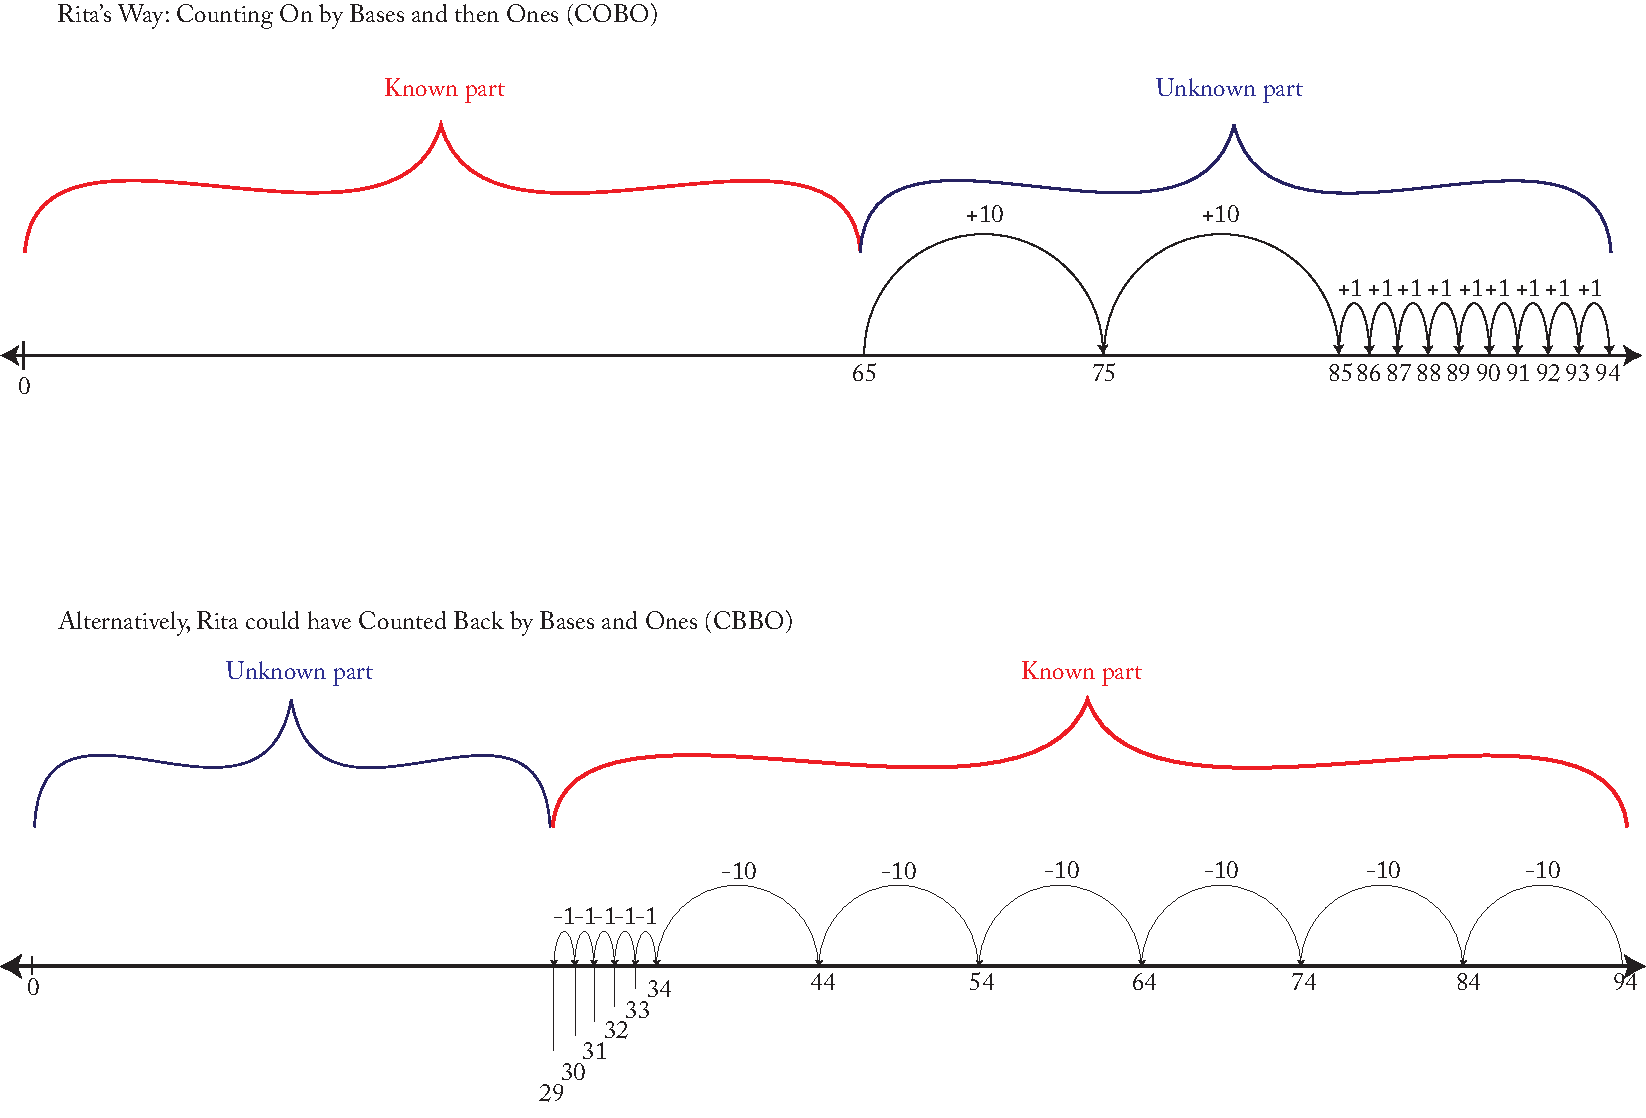
\includegraphics[width=.8\textwidth]{images/Easy_Pictures/SAR_SUB_COBO/PDF/SAR_SUB_COBO_CBBO.pdf}

\noindent \textbf{Notation Representing Rita's Solution:}
\begin{align*}
    65 + (10) &= 75\\
    75 + (10) &= 85\\
    85 + 1 + 1 + 1 + 1 + 1 + 1 + 1 + 1 + 1 &= 94\\
    10 + 10 + 1 + 1 + 1 + 1 + 1 + 1 + 1 + 1 + 1 &= 29
    \end{align*}
    

\subsubsection*{Description of Strategy:}

 \textbf{Objective:} Description of Counting On by Bases and Then Ones (COBO)
 Begin with one of the numbers. Break the other number into its base units and its ones. Then, “count on” by adding each base unit one at a time, followed by each individual one.
 
 Why are number lines useful for demonstrating this strategy?
 COBO is essentially a jump strategy—you start at one number and make “jumps” equal to the other number’s base units, then add in the remaining ones. Number lines are ideal because they visually display jumps of varying lengths and directions. They serve as a picture of the process: a jump representing a full base is clearly larger (by a factor of the base) than a jump of a single unit.
 
 Good number line illustrations should:
\begin{itemize}
 \item Clearly represent the relative sizes of the jumps—each base jump should be exactly as many times larger than a single-unit jump as the base indicates, with all base jumps the same size and all one-unit jumps identical.
 \item Indicate the position of 0, or mark a break if that portion of the line isn’t drawn to scale.
 \item Use arrows to indicate direction—when adding, the jumps go to the right (or upward); when subtracting, they go to the left (or downward).
 \item Mark all landing points clearly—the numbers you would speak aloud when counting on by bases and then ones, just as Lauren demonstrated.
\end{itemize}

\subsubsection*{Corrected Automata (Register Machines)}

We define two distinct Register Machines to model these strategies accurately.

\paragraph{Automaton 1: COBO (Missing Addend)}
This machine models starting at S and counting up to M.
\begin{longtable}{|l|l|l|l|}
\hline
\textbf{State} & \textbf{Condition} & \textbf{Next State} & \textbf{Action} \\
\hline
\endhead
$q_{init}$ & - & $q_{add\_bases}$ & CurrentValue=S; Distance=0 \\
\hline
$q_{add\_bases}$ & **CurrentValue + Base <= M** & $q_{add\_bases}$ & CurrentValue+=Base; Distance+=Base \\
\hline
$q_{add\_bases}$ & (Overshoot Detected) & $q_{add\_ones}$ & - \\
\hline
$q_{add\_ones}$ & **CurrentValue < M** & $q_{add\_ones}$ & CurrentValue+=1; Distance+=1 \\
\hline
$q_{add\_ones}$ & (Target Reached) & $q_{accept}$ & Result=Distance \\
\hline
\end{longtable}

\paragraph{Automaton 2: CBBO (Take Away)}
This machine models starting at M and counting back by S.
\begin{longtable}{|l|l|l|l|}
\hline
\textbf{State} & \textbf{Condition} & \textbf{Next State} & \textbf{Action} \\
\hline
\endhead
$q_{init}$ & - & $q_{sub\_bases}$ & CurrentValue=M; Decompose S (BC, OC) \\
\hline
$q_{sub\_bases}$ & **BaseCounter (BC) > 0** & $q_{sub\_bases}$ & CurrentValue-=Base; BC-=1 \\
\hline
$q_{sub\_bases}$ & (Bases Exhausted) & $q_{sub\_ones}$ & - \\
\hline
$q_{sub\_ones}$ & **OneCounter (OC) > 0** & $q_{sub\_ones}$ & CurrentValue-=1; OC-=1 \\
\hline
$q_{sub\_ones}$ & (Ones Exhausted) & $q_{accept}$ & Result=CurrentValue \\
\hline
\end{longtable}

\subsubsection*{Python Implementation and Test}

\begin{lstlisting}[language=Python]
import pandas as pd

class SubtractionIterativeAutomaton:
    """Base class for iterative subtraction strategies."""
    def __init__(self, M, S, Base=10):
        self.M = M # Minuend (Whole)
        self.S = S # Subtrahend (Known Part)
        self.BaseUnit = Base
        self.history = []
        self.state = 'q_start'
        self.Result = 0

        # Initialize registers for consistent history recording
        self.CurrentValue = 0

        if S > M:
            self.state = 'q_error'
            # Manually record error history as derived class registers may not be initialized yet
            self.history.append({'State': 'q_error', 'Interpretation': f"Error: Subtrahend ({S}) > Minuend ({M})."})

    def _record_history(self, interpretation, **kwargs):
        # Standardize history recording
        record = {'State': self.state, 'Interpretation': interpretation}
        # Include core registers if they exist in the specific strategy
        if hasattr(self, 'CurrentValue'):
            record['CV'] = self.CurrentValue
        if hasattr(self, 'Distance'):
            record['Dist'] = self.Distance
        if hasattr(self, 'BaseCounter'):
            record['BC'] = self.BaseCounter
        if hasattr(self, 'OneCounter'):
            record['OC'] = self.OneCounter

        record.update(kwargs) # Add any specific overrides
        self.history.append(record)

    def transition(self, next_state):
        self.state = next_state

    def run(self):
        while self.state not in ['q_accept', 'q_error']:
            executor = getattr(self, f"execute_{self.state}", self.execute_error)
            executor()
        return self.Result

    def execute_error(self):
        if self.state != 'q_error':
            self._record_history(f"Error: Entered unknown state {self.state}")
            self.transition('q_error')

    def execute_q_start(self):
        # Common start state
        self._record_history("Start.")
        self.transition('q_init')

    def display_history(self):
        print(f"\n--- Subtraction History ({self.M} - {self.S}) | Strategy: {self.strategy_name} ---")
        df = pd.DataFrame(self.history)
        if not df.empty:
             # Define desired column order and filter existing columns
            cols_order = ['State', 'Interpretation', 'CV', 'Dist', 'BC', 'OC']
            cols = [col for col in cols_order if col in df.columns]
            df = df[cols].fillna('')
        print(df.to_markdown(index=False))

# =============================================================================
# Strategy 1: COBO (Counting On - Missing Addend)
# =============================================================================

class COBO_MissingAddend(SubtractionIterativeAutomaton):
    """
    COBO (Counting On): Start at S, count up to M iteratively. Result is distance.
    Models Rita's strategy.
    """
    strategy_name = "COBO (Counting On - Missing Addend)"

    def __init__(self, M, S, Base=10):
        super().__init__(M, S, Base)
        self.Distance = 0
        self.Target = self.M

    def execute_q_init(self):
        self.CurrentValue = self.S
        self.Distance = 0
        self._record_history(f"Initialize at S ({self.S}). Target is M ({self.M}).")
        self.transition('q_add_bases')

    def execute_q_add_bases(self):
        """Iteratively add bases, checking for overshoot."""
        # Condition: Can add a base without overshooting M
        if self.CurrentValue + self.BaseUnit <= self.Target:
            self.CurrentValue += self.BaseUnit
            self.Distance += self.BaseUnit
            self._record_history(f"Count on by base (+{self.BaseUnit}). New Value={self.CurrentValue}.")
            # Stay in q_add_bases
        # Condition: Adding a base would overshoot
        else:
            self._record_history("Next base overshoots target. Switching to ones.")
            self.transition('q_add_ones')

    def execute_q_add_ones(self):
        """Iteratively add ones until M is reached."""
        # Condition: Not yet reached M
        if self.CurrentValue < self.Target:
            self.CurrentValue += 1
            self.Distance += 1
            self._record_history(f"Count on by one (+1). New Value={self.CurrentValue}.")
            # Stay in q_add_ones
        # Condition: Reached M
        else:
            self.Result = self.Distance
            self._record_history(f"Target reached. Result (Distance) = {self.Result}.")
            self.transition('q_accept')

# =============================================================================
# Strategy 2: CBBO (Counting Back - Take Away)
# =============================================================================

class CBBO_TakeAway(SubtractionIterativeAutomaton):
    """
    CBBO (Counting Back): Start at M, subtract S iteratively. Result is final position.
    Models the alternative strategy diagram.
    """
    strategy_name = "CBBO (Counting Back - Take Away)"

    def __init__(self, M, S, Base=10):
        super().__init__(M, S, Base)
        self.BaseCounter = 0
        self.OneCounter = 0

    def execute_q_init(self):
        self.CurrentValue = self.M
        # Decompose S into iterative counts
        self.BaseCounter = self.S // self.BaseUnit
        self.OneCounter = self.S % self.BaseUnit
        self._record_history(f"Initialize at M ({self.M}). Decompose S ({self.S}): {self.BaseCounter} bases, {self.OneCounter} ones.")
        self.transition('q_sub_bases')

    def execute_q_sub_bases(self):
        """Iteratively subtract bases."""
        if self.BaseCounter > 0:
            self.CurrentValue -= self.BaseUnit
            self.BaseCounter -= 1
            self._record_history(f"Count back by base (-{self.BaseUnit}). New Value={self.CurrentValue}.")
        else:
            self._record_history("Bases finished. Switching to ones.")
            self.transition('q_sub_ones')

    def execute_q_sub_ones(self):
        """Iteratively subtract ones."""
        if self.OneCounter > 0:
            self.CurrentValue -= 1
            self.OneCounter -= 1
            self._record_history(f"Count back by one (-1). New Value={self.CurrentValue}.")
        else:
            self.Result = self.CurrentValue
            self._record_history(f"Subtraction finished. Result (Final Position) = {self.Result}.")
            self.transition('q_accept')

# =============================================================================
# Testing (Example: 94 - 65)
# =============================================================================

M_test = 94
S_test = 65

# Test COBO (Rita's actual strategy)
print("=== Testing Rita's Strategy (COBO) ===")
cobo = COBO_MissingAddend(M=M_test, S=S_test)
cobo.run()
cobo.display_history()

# Test CBBO (The alternative strategy shown in the diagram)
print("\n=== Testing Alternative Strategy (CBBO) ===")
cbbo = CBBO_TakeAway(M=M_test, S=S_test)
cbbo.run()
cbbo.display_history()
\end{lstlisting}

\printbibliography
\end{document}